\documentclass[11pt]{article}

\usepackage[margin=1in]{geometry}
\usepackage{amsmath,amssymb,amsthm}
\usepackage{graphicx}
\usepackage{booktabs}
\usepackage{hyperref}
\usepackage{natbib}
\usepackage{xcolor}

%% Macros shared across sections
\newcommand{\E}{\mathbb{E}}
\newcommand{\Tub}{T_{\text{UB}}}
\newcommand{\Tbot}{T_{\text{bot}}}
\newcommand{\Tul}{T_{\text{UL}}}
\newcommand{\Tlh}{T_{\text{LH}}}
\newcommand{\Tsim}{T_{\text{sim}}}
\newcommand{\Smax}{S_{\max}}
\newcommand{\mumin}{\mu_{\min}}
\newcommand{\mumax}{\mu_{\max}}

\title{Two Approximations for the Mean Response Time of\\
       Heterogeneous Two-Queue Fork-Join Systems}
\author{Anonymous Author}
\date{}

\begin{document}
\maketitle

\begin{abstract}
We develop and compare two closed-form approximations for the mean response time
of a heterogeneous two-queue M/M/1 fork-join system, in which the two servers
may have different service rates $\mu_1 \geq \mu_2$.
The first approximation, $\Tul$, interpolates between a known independent upper
bound and a bottleneck lower bound, using the average server utilization as the
interpolation weight.
The second approximation, $\Tlh$, is derived from the Reiman--Simon light-heavy
traffic interpolation framework: it matches the exact light-traffic value and a
heavy-traffic limit $h(r)$ that depends on the heterogeneity ratio
$r = \mu_1/\mu_2$.
Both approximations recover the exact Nelson--Tantawi formula in the homogeneous
case ($\mu_1 = \mu_2$) and are validated against discrete-event simulation across
a wide range of loads and heterogeneity levels, with errors below $2.5\%$.
\end{abstract}

\section{Introduction}
\label{sec:intro}

Fork-join queueing systems model the parallel execution of tasks that must
all complete before a job can proceed.
A job arrives, \emph{forks} into $n$ tasks dispatched to $n$ parallel servers,
and \emph{joins}---departs---only when the last task finishes.
This synchronization constraint makes fork-join queues substantially harder
to analyze than independent queues, because the job response time is the
\emph{maximum} of the task sojourn times, and those times are stochastically
dependent.

We study the canonical case of $n = 2$ servers with Poisson arrivals at
rate $\lambda$ and exponential service times at rates $\mu_1$ and $\mu_2$,
with $\mu_1 \geq \mu_2$ without loss of generality.
The primary performance measure is the mean job response time:
\begin{equation}
  T = \E[\max(R_1, R_2)],
\end{equation}
where $R_i$ is the sojourn time (waiting plus service) of a task at server~$i$.
The system is stable when $\lambda < \mumin \equiv \mu_2$.

For the \emph{homogeneous} case $\mu_1 = \mu_2 = \mu$, Nelson and
Tantawi~\citep{Nelson1988} derived the exact closed-form result
\begin{equation}
  \label{eq:nelson-tantawi}
  T_2^{\mathrm{hom}} = \frac{12 - \rho}{8(\mu - \lambda)},
  \qquad \rho = \frac{\lambda}{\mu},
\end{equation}
using a light-heavy traffic interpolation argument.
For \emph{heterogeneous} servers ($\mu_1 \neq \mu_2$), the exact joint
distribution of $(R_1, R_2)$ is not available in closed form.
Flatto and Hahn~\citep{Flatto1984,Flatto1985} obtained the exact generating
function via an elliptic function parametrization, but extracting the mean
response time requires solving a boundary value problem and does not yield
a tractable expression.
Bounds, heavy-traffic asymptotics, and distributional
approximations have been developed~\citep{Baccelli1989,Kemper2012,Rizk2015,Mohanty2024},
but no simple closed-form approximation covering the full range of loads and
heterogeneity levels has previously been established.

In this paper we propose and analyze two complementary closed-form
approximations:
\begin{enumerate}
\item \textbf{$\Tul$ (upper-lower bound interpolation):}
      A convex combination of the independent upper bound $\Tub$ and the
      bottleneck lower bound $\Tbot$, weighted by the average utilization.
      It is guaranteed to lie within the bounds and is exact for the
      homogeneous case.
\item \textbf{$\Tlh$ (light-heavy traffic interpolation):}
      A rational approximation in the bottleneck utilization, derived from the
      Reiman--Simon framework~\citep{Reiman1988} as described
      in~\citep{Squillante2026}.
      It matches the exact light-traffic value and a heavy-traffic factor
      $h(r) = 1 + \tfrac{3}{8}\,r^{-\beta}$ that smoothly interpolates
      between the homogeneous limit ($h = 11/8$) and the bottleneck limit
      ($h \to 1$) as a function of the heterogeneity ratio $r = \mu_1/\mu_2$.
\end{enumerate}

Both approximations reduce exactly to the Nelson--Tantawi result
(\ref{eq:nelson-tantawi}) in the homogeneous case, exhibit the correct
singularity structure in heavy traffic, and agree with simulation to within
$2.5\%$ across all tested scenarios.

The remainder of the paper is organized as follows.
Section~\ref{sec:bounds} reviews known upper and lower bounds.
Sections~\ref{sec:approx-ul} and~\ref{sec:approx-lh} derive the two
approximations.
Section~\ref{sec:validation} presents simulation validation.
Section~\ref{sec:discussion} discusses the relationship between the two
methods, their limitations, and connections to prior work.
Section~\ref{sec:conclusion} concludes.

\section{Bounds}
\label{sec:bounds}

We introduce notation used throughout.
Let $\rho_i = \lambda/\mu_i$ denote the utilization of server~$i$,
$T_i = 1/(\mu_i - \lambda)$ the mean M/M/1 sojourn time at server~$i$,
and $r = \mumax/\mumin = \mu_1/\mu_2 \geq 1$ the heterogeneity ratio.

\subsection{Independent Upper Bound}

Since the two task sojourn times $R_1$ and $R_2$ share a common Poisson
arrival stream, they are positively correlated.
Positive correlation reduces the expected maximum below what it would be
under independence~\citep{Baccelli1989}.
Treating $R_i$ as independent M/M/1 sojourn times with rates $\mu_i - \lambda$
yields:
\begin{equation}
  \label{eq:tub}
  \Tub = \frac{1}{\mu_1 - \lambda} + \frac{1}{\mu_2 - \lambda}
         - \frac{1}{\mu_1 + \mu_2 - 2\lambda},
\end{equation}
which satisfies $T \leq \Tub$.
The formula follows from $\E[\max(X_1,X_2)] = \E[X_1] + \E[X_2] - \E[\min(X_1,X_2)]$
applied to independent exponentials with rates $\mu_i - \lambda$.

\subsection{Bottleneck Lower Bound}

By Jensen's inequality and the convexity of the max function:
\begin{equation}
  \label{eq:tbot}
  \Tbot = \max(T_1, T_2) = \frac{1}{\mumin - \lambda} \;\leq\; T.
\end{equation}
This is simply the mean sojourn time of the bottleneck M/M/1 queue.

\subsection{Gap Between the Bounds}

In the homogeneous case ($r = 1$), $\Tub = \tfrac{3}{2}T_1$ and
$\Tbot = T_1$, giving a $50\%$ gap.
The exact value $T_2^{\mathrm{hom}} = \tfrac{12-\rho}{8}\,T_1$ lies strictly
between them, approaching $\Tub$ at light load ($\rho \to 0$, ratio $T_2^{\mathrm{hom}}/\Tub \to 1$)
and $\Tbot$ in heavy traffic ($\rho \to 1$, ratio $T_2^{\mathrm{hom}}/\Tbot \to 11/8$).

For $r > 1$, the gap narrows: as $r \to \infty$, both $\Tub$ and $\Tbot$
converge to $1/(\mumin - \lambda)$ from above, so the bounds become tight and
the system is well approximated by a single bottleneck M/M/1 queue.

\subsection{Summary}

For all stable parameters ($\lambda < \mumin$):
\begin{equation}
  \Tbot \;\leq\; T \;\leq\; \Tub.
\end{equation}
Any good approximation should lie within this interval and recover the known
endpoint behaviors.

\section{Approximation 1: Upper-Lower Bound Interpolation}
\label{sec:approx-ul}

\subsection{Derivation}

We seek a convex combination of $\Tub$ and $\Tbot$ that:
\begin{enumerate}
  \item recovers the Nelson--Tantawi result~\eqref{eq:nelson-tantawi} when
        $\mu_1 = \mu_2$,
  \item approaches $\Tub$ in light traffic ($\lambda \to 0$),
  \item approaches $\Tbot$ in heavy traffic ($\lambda \to \mumin$), and
  \item always satisfies $\Tbot \leq T \leq \Tub$.
\end{enumerate}

Write $\Tul = (1-\alpha)\Tub + \alpha\Tbot$ and determine $\alpha$ from
condition~1.
In the homogeneous case, $\Tub = \tfrac{3}{2}T_1$ and $\Tbot = T_1$, so:
\begin{equation}
  \frac{12-\rho}{8}T_1 = (1-\alpha)\tfrac{3}{2}T_1 + \alpha T_1
  \;\;\Longrightarrow\;\;
  \alpha = \frac{3/2 - (12-\rho)/8}{3/2 - 1} = \frac{\rho}{4}.
\end{equation}
The natural heterogeneous generalization replaces $\rho$ with the average
utilization $\bar{\rho} = (\rho_1+\rho_2)/2$, giving:
\begin{equation}
  \alpha = \frac{\bar{\rho}}{4} = \frac{\rho_1 + \rho_2}{8}.
\end{equation}

\subsection{The Formula}

\begin{equation}
  \label{eq:tul}
  \boxed{\Tul = \left(1 - \frac{\rho_1+\rho_2}{8}\right)\Tub
                + \frac{\rho_1+\rho_2}{8}\,\Tbot,}
\end{equation}
where $\Tub$ and $\Tbot$ are given by~\eqref{eq:tub} and~\eqref{eq:tbot}.

\subsection{Verification: Homogeneous Case}

When $\mu_1 = \mu_2 = \mu$:
$\rho_1 = \rho_2 = \rho$,
$\Tub = \tfrac{3}{2}T_1$,
$\Tbot = T_1$,
$\alpha = \rho/4$.
Substituting:
\begin{equation}
  \Tul = \left(1 - \frac{\rho}{4}\right)\frac{3}{2}T_1 + \frac{\rho}{4}T_1
       = \frac{3}{2}T_1 - \frac{3\rho}{8}T_1 + \frac{\rho}{4}T_1
       = \frac{12-\rho}{8}T_1 = T_2^{\mathrm{hom}}. \quad \checkmark
\end{equation}

\subsection{Properties}

\begin{table}[h]
\centering
\caption{Properties of $\Tul$.}
\label{tab:properties-ul}
\begin{tabular}{@{}ll@{}}
\toprule
Property & Status \\
\midrule
Exact for homogeneous case ($\mu_1 = \mu_2$) & \checkmark \\
Satisfies $\Tbot \leq \Tul \leq \Tub$ & \checkmark\quad ($0 \leq \alpha \leq 1/4 < 1$) \\
Light traffic limit ($\lambda \to 0$) & \checkmark\quad ($\alpha \to 0$, so $\Tul \to \Tub$) \\
Heavy traffic limit ($\lambda \to \mumin$) & \checkmark\quad ($\Tbot$ diverges; $\Tul/\Tbot \to 1$) \\
No free parameters & \checkmark \\
\bottomrule
\end{tabular}
\end{table}

The weight $\alpha \leq 1/4$ ensures $\Tul$ always lies strictly within the
bounds (unless $\alpha = 0$, i.e., $\lambda = 0$).
The formula is symmetric in $\mu_1$ and $\mu_2$ via the average utilization,
consistent with the symmetry of the original problem.

\section{Approximation 2: Light-Heavy Traffic Interpolation}
\label{sec:approx-lh}

\subsection{The Reiman--Simon Framework}

Reiman and Simon~\citep{Reiman1988} developed a systematic method for
constructing rational approximations to performance quantities in Markovian
queueing networks, exploiting exact light-traffic derivatives and a
heavy-traffic limit.
For a scalar performance measure $f(\rho)$ with normalizing denominator
$d(\rho) = \mumin(1-\rho)$, the $n$-th order approximation takes the form
\begin{equation}
  \tilde{f}(\rho) = \frac{a_n\rho^n + \cdots + a_1\rho + a_0}{\mumin(1-\rho)},
\end{equation}
where the $n+1$ coefficients $\{a_i\}$ are matched to the $n$ derivatives of
$f$ at $\rho = 0$ and the heavy-traffic constant
$h = \lim_{\rho\to1}\mumin(1-\rho)f(\rho)$~\citep{Squillante2026}.

We apply this framework to $T(\rho)$ with a first-order (linear) numerator,
yielding two matching conditions:

\subsection{Matching Condition 1: Light-Traffic Value}

At $\lambda = 0$, all queues are empty.
The task service times $X_i \sim \mathrm{Exp}(\mu_i)$ are independent and
$T(0) = \E[\max(X_1, X_2)]$.
Using the identity $\E[\max(X_1,X_2)] = \E[X_1]+\E[X_2]-\E[\min(X_1,X_2)]$
and the fact that $\min(X_1,X_2) \sim \mathrm{Exp}(\mu_1+\mu_2)$:
\begin{equation}
  \label{eq:T0}
  T_0 \;=\; T(\rho=0) \;=\; \frac{1}{\mu_1} + \frac{1}{\mu_2}
      - \frac{1}{\mu_1 + \mu_2}.
\end{equation}
Matching $\tilde{T}(0) = T_0$ gives:
\begin{equation}
  \label{eq:a0}
  a_0 = \mumin \cdot T_0.
\end{equation}

\subsection{Matching Condition 2: Heavy-Traffic Limit}

Define the heavy-traffic constant:
\begin{equation}
  h = \lim_{\rho \to 1} \mumin(1-\rho)\cdot T(\rho).
\end{equation}
Matching this in $\tilde{T}$ gives $a_0 + a_1 = h$, hence $a_1 = h - a_0$.

\subsection{The Heavy-Traffic Factor $h(r)$}

The value of $h$ depends on the heterogeneity ratio $r = \mumax/\mumin \geq 1$.

\paragraph{Homogeneous case ($r = 1$).}
When $\mu_1 = \mu_2 = \mu$, both servers saturate simultaneously as
$\lambda \to \mu$.
The Nelson--Tantawi formula gives:
\begin{equation}
  h = \lim_{\rho\to1}\mu(1-\rho)\cdot\frac{12-\rho}{8(\mu-\lambda)}
    = \lim_{\rho\to1}\frac{12-\rho}{8} = \frac{11}{8}.
\end{equation}

\paragraph{Heterogeneous case ($r > 1$).}
As $\lambda \to \mumin$, the bottleneck server saturates while the faster
server's utilization approaches $\lambda/\mumax = 1/r < 1$.
The faster server's sojourn time remains bounded, so the bottleneck dominates
and $T(\rho) \sim 1/(\mumin - \lambda)$, giving $h \to 1$.

\paragraph{Proposed model.}
We interpolate between these two limits with the power-law factor:
\begin{equation}
  \label{eq:h}
  h(r) = 1 + \frac{3}{8}\,r^{-\beta}, \qquad r \geq 1,\quad \beta > 0.
\end{equation}
This satisfies $h(1) = 11/8$ for all $\beta$, and $h(r) \to 1$ as
$r \to \infty$.
The parameter $\beta$ controls the rate of decay; larger $\beta$ means the
correction vanishes more rapidly with heterogeneity.

\paragraph{Calibration.}
Simulation data reveal that the transition from $h = 11/8$ to $h \approx 1$
is very sharp in practice: the effective heavy-traffic constant is already
$h \approx 1.008$ at $r = 1.5$.
Matching this observation to~\eqref{eq:h} gives
$\beta = \log(0.375/0.008)/\log(1.5) \approx 9.5$,
consistent with a default of $\beta = 10$.

\subsection{The Formula}

Substituting $a_0$ and $a_1 = h(r) - a_0$ into the first-order template and
collecting terms (with $\rho = \lambda/\mumin$), the response time separates
into its light-traffic value plus a single load-dependent term:
\begin{equation}
  \label{eq:tlh}
  \boxed{\Tlh = T_0 + \frac{\lambda}{\mumin - \lambda}\cdot\frac{h(r)}{\mumin},}
\end{equation}
where $T_0$ is given by~\eqref{eq:T0} and $h(r)$ by~\eqref{eq:h}.
The first term is the exact light-traffic limit; the second carries the
heavy-traffic singularity at $\lambda \to \mumin$, scaled by $h(r)$.

\subsection{Verification: Homogeneous Case}

When $\mu_1 = \mu_2 = \mu$ (so $r = 1$, $h = 11/8$, $T_0 = 3/(2\mu)$):
\begin{equation}
  a_0 = \mu \cdot \frac{3}{2\mu} = \frac{3}{2},
  \qquad
  a_1 = \frac{11}{8} - \frac{3}{2} = -\frac{1}{8}.
\end{equation}
\begin{equation}
  \Tlh = \frac{3/2 - \rho/8}{\mu(1-\rho)}
       = \frac{12 - \rho}{8(\mu - \lambda)}
       = T_2^{\mathrm{hom}}. \quad \checkmark
\end{equation}
This recovery holds for every $\rho \in [0,1)$, regardless of $\beta$,
because $h(1) = 11/8$ is exact.

\subsection{Properties}

\begin{table}[h]
\centering
\caption{Properties of $\Tlh$.}
\label{tab:properties-lh}
\begin{tabular}{@{}ll@{}}
\toprule
Property & Status \\
\midrule
Exact for homogeneous case ($\mu_1 = \mu_2$) & \checkmark\quad (for any $\beta$) \\
Light traffic limit ($\lambda \to 0$) & \checkmark\quad ($\Tlh \to T_0$) \\
Heavy traffic singularity ($\lambda \to \mumin$) & \checkmark\quad ($\Tlh \sim h(r)/(\mumin-\lambda)$) \\
Bound compliance $\Tbot \leq \Tlh \leq \Tub$ & Not guaranteed \\
Tunable parameter & $\beta$ (default 10) \\
\bottomrule
\end{tabular}
\end{table}

\subsection{First-Order Extension: Enhanced $\Tlh$}
\label{sec:approx-lhe}

The current $\Tlh$ uses a linear numerator matched to two conditions:
the light-traffic value $T_0 = f^{(0)}(0)$ and the heavy-traffic constant $h$.
The Reiman--Simon framework accommodates a \emph{quadratic} numerator by
adding the first light-traffic derivative as a third matching
condition~\citep{Squillante2026}, which we denote
$T_0' \equiv f^{(1)}(0) = \frac{dT}{d\lambda}\big|_{\lambda=0}$.
We call the resulting enhanced approximation $\Tlhe$.

\subsection{First Light-Traffic Derivative}
\label{sec:f1}

Following~\citep{Squillante2026}, the first derivative of the mean response
time with respect to $\lambda$ at $\lambda = 0$ is:
\begin{equation}
  \label{eq:f1}
  T_0' = f^{(1)}(0) = \frac{1}{\mumin^2} + \frac{1}{\mumax^2}
             - \frac{2}{(\mumin+\mumax)^2}
             - \frac{2\,\mumin\,\mumax}{(\mumin+\mumax)^4}.
\end{equation}
This is derived by considering the sojourn time of a tagged job conditioned
on exactly one background arrival at time $t \in (-\infty, \infty)$,
analyzing the resulting joint service-time distribution, and integrating
over $t$.

\subsection{The Enhanced Formula}
\label{sec:tlhe}

With three matching conditions---$T_0 = f^{(0)}(0)$, $T_0'$, and $h$---the
interpolating polynomial $\tilde{g}(\rho) = c_2\rho^2 + c_1\rho + c_0$
for $g(\rho) = \mumin(1-\rho)T(\rho)$ has coefficients:
\begin{align}
  c_0 &= \mumin \cdot T_0, \label{eq:c0} \\
  c_1 &= \mumin^2 \cdot T_0' - \mumin \cdot T_0, \label{eq:c1} \\
  c_2 &= h - c_1 - c_0. \label{eq:c2}
\end{align}
Here $c_0$ is identical to $a_0$ in~\eqref{eq:a0}; $c_1$ is determined by
the first derivative rather than by $h$ alone; and $c_2$ absorbs the
remaining difference to satisfy the heavy-traffic condition.
Inverting the scaling gives the quadratic-numerator form
\begin{equation*}
  \Tlhe = \frac{c_2\,\rho^2 + c_1\,\rho + c_0}{\mumin(1-\rho)},
  \qquad \rho = \lambda/\mumin.
\end{equation*}
Substituting the coefficients~\eqref{eq:c0}--\eqref{eq:c2} and comparing
with~\eqref{eq:tlh}, the difference $\Tlhe - \Tlh$ is non-singular---the
$(1-\rho)$ denominators cancel---leaving a single bounded correction to
$\Tlh$:
\begin{equation}
  \label{eq:tlhe}
  \boxed{\Tlhe = \Tlh + \lambda\left(T_0' - \frac{h(r)}{\mumin^2}\right),}
\end{equation}
where $\Tlh$ is given by~\eqref{eq:tlh}, $T_0'$ by~\eqref{eq:f1}, and $h(r)$
by~\eqref{eq:h}.
The correction is linear in $\lambda$ and shifts $\Tlh$ by a finite amount at
every load, vanishing exactly when $T_0' = h(r)/\mumin^2$.

\subsection{Verification: Homogeneous Case}

When $\mu_1 = \mu_2 = \mu$ (so $\mumin = \mumax = \mu$), the first derivative is
\begin{equation}
  T_0' = \frac{2}{\mu^2} - \frac{2}{4\mu^2} - \frac{2\mu^2}{16\mu^4}
       = \frac{11}{8\mu^2}.
\end{equation}
With $h(1) = 11/8$, the correction bracket in~\eqref{eq:tlhe} is
\begin{equation}
  T_0' - \frac{h(1)}{\mu^2} = \frac{11}{8\mu^2} - \frac{11}{8\mu^2} = 0.
\end{equation}
The correction vanishes identically, so $\Tlhe = \Tlh$, which recovers the
Nelson--Tantawi formula~\eqref{eq:nelson-tantawi} for all $\rho$
(equivalently, $c_2 = h - c_1 - c_0 = 0$).
The enhancement is automatically inactive in the homogeneous case,
regardless of $\beta$.

\subsection{Properties of the Enhanced Approximation}

\begin{table}[h]
\centering
\caption{Properties of $\Tlhe$.}
\label{tab:properties-lhe}
\begin{tabular}{@{}ll@{}}
\toprule
Property & Status \\
\midrule
Exact for homogeneous case ($\mu_1 = \mu_2$) & \checkmark\quad (for any $\beta$; $c_2 = 0$) \\
Light traffic limit ($\lambda \to 0$) & \checkmark\quad ($\Tlhe \to T_0$) \\
First light-traffic derivative matched & \checkmark \\
Heavy traffic singularity ($\lambda \to \mumin$) & \checkmark\quad ($\Tlhe \sim h(r)/(\mumin-\lambda)$) \\
Bound compliance $\Tbot \leq \Tlhe \leq \Tub$ & Not guaranteed \\
Numerator degree & 2 (quadratic) \\
Tunable parameter & $\beta$ (default 10) \\
\bottomrule
\end{tabular}
\end{table}

\section{Simulation Validation}
\label{sec:validation}

All three approximations were validated against discrete-event simulation of the
two-queue fork-join system.
Each scenario used 20\,M jobs with a 500\,K-job warmup period, repeated over
5 independent random seeds; the reported $\Tsim$ is the grand mean and the
95\% confidence interval is computed via the $t$-distribution across seeds
($\mathrm{df}=4$).
Results for $\Tul$~\eqref{eq:tul} and $\Tlh$~\eqref{eq:tlh} (with $\beta = 10$)
are shown in Table~\ref{tab:results} alongside the theoretical bounds.
Table~\ref{tab:results-lhe} compares $\Tlh$ and the enhanced approximation
$\Tlhe$~\eqref{eq:tlhe}.

\begin{table}[ht]
\centering
\caption{Approximations vs.\ simulation for heterogeneous two-queue fork-join.
         $\Tsim$ is the grand mean over 5 seeds; $\pm$ is the 95\% CI half-width.
         Errors are $(T_{\text{approx}} - \Tsim)/\Tsim \times 100\%$.}
\label{tab:results}
\resizebox{\textwidth}{!}{%
\begin{tabular}{@{}ccccccccccc@{}}
\toprule
$\mu_1$ & $\mu_2$ & $\lambda$ & $\rho_2$ & $\Tbot$
        & $\Tsim$ & $\pm$95\%\,CI & $\Tul$ & Err & $\Tlh$ & Err \\
\midrule
1.0 & 1.0 & 0.3 & 0.30 & 1.429 & 2.089 & 0.001 & 2.089 & $0.00\%$ & 2.089 & $0.00\%$ \\
1.0 & 1.0 & 0.6 & 0.60 & 2.500 & 3.562 & 0.004 & 3.562 & $+0.01\%$ & 3.562 & $+0.01\%$ \\
1.0 & 1.0 & 0.9 & 0.90 & 10.000 & 13.892 & 0.082 & 13.875 & $-0.12\%$ & 13.875 & $-0.12\%$ \\
\midrule
1.0 & 1.5 & 0.3 & 0.20 & 1.429 & 1.707 & 0.001 & 1.716 & $+0.57\%$ & 1.698 & $-0.51\%$ \\
1.0 & 1.5 & 0.6 & 0.40 & 2.500 & 2.768 & 0.003 & 2.799 & $+1.13\%$ & 2.776 & $+0.31\%$ \\
1.0 & 1.5 & 0.9 & 0.60 & 10.000 & 10.142 & 0.083 & 10.193 & $+0.50\%$ & 10.325 & $+1.80\%$ \\
\midrule
1.0 & 2.0 & 0.3 & 0.15 & 1.429 & 1.583 & 0.001 & 1.590 & $+0.44\%$ & 1.595 & $+0.75\%$ \\
1.0 & 2.0 & 0.6 & 0.30 & 2.500 & 2.624 & 0.003 & 2.641 & $+0.64\%$ & 2.667 & $+1.64\%$ \\
1.0 & 2.0 & 0.9 & 0.45 & 10.000 & 10.050 & 0.083 & 10.063 & $+0.12\%$ & 10.170 & $+1.19\%$ \\
\midrule
1.0 & 3.0 & 0.6 & 0.20 & 2.500 & 2.548 & 0.003 & 2.554 & $+0.22\%$ & 2.583 & $+1.39\%$ \\
1.0 & 5.0 & 0.6 & 0.12 & 2.500 & 2.516 & 0.003 & 2.517 & $+0.04\%$ & 2.533 & $+0.68\%$ \\
\bottomrule
\end{tabular}%
}
\end{table}

\paragraph{Homogeneous case ($\mu_1 = \mu_2 = 1.0$).}
Both approximations recover the Nelson--Tantawi formula~\eqref{eq:nelson-tantawi}
by construction; residual errors ($\leq 0.12\%$) are simulation noise.
At $\lambda = 0.9$ the CI half-width is $\pm 0.082$, reflecting the heavy-tailed
response-time distribution near saturation; the analytical value $13.875$ lies
well within this interval.

\paragraph{Moderate heterogeneity ($r = 1.5$).}
$\Tul$ shows consistent positive errors ($+0.50\%$ to $+1.13\%$) across all
loads.
$\Tlh$ is more accurate at low and moderate load, but reaches $+1.80\%$ at
heavy load ($\rho_2 = 0.6$).
The wider CIs at $\lambda = 0.9$ (half-width $\pm 0.083$) indicate substantial
variance in the heavy-load regime; a short-run single-seed estimate is biased
low near saturation, illustrating the
importance of long runs and multiple seeds in this regime.

\paragraph{High heterogeneity ($r \geq 2$).}
$\Tul$ errors fall below $0.64\%$ and improve further as $r$ increases
($\leq 0.04\%$ at $r = 5$).
$\Tlh$ errors are slightly larger (up to $+1.64\%$ at $r = 2$).
CIs are tight at low-to-moderate load ($\leq \pm 0.003$ for $\rho_2 \leq 0.45$)
and widen to $\pm 0.083$ near saturation ($\lambda = 0.9$); relative to
$\Tsim \approx 10$ this is still below $1\%$, confirming that 20\,M jobs over
5 seeds provide well-converged estimates in this regime.
As $r \to \infty$, both approximations converge to $\Tbot$.

Figure~\ref{fig:vs-load} plots the two approximations, bounds, and simulation
as functions of load for $\mu_1 = 1.0$, $\mu_2 = 2.0$.
Both $\Tul$ and $\Tlh$ track the simulation closely across the full load
range, lying between the theoretical bounds.
Figure~\ref{fig:vs-hetero} shows the same quantities as a function of
the heterogeneity ratio $\mu_2/\mu_1$ at fixed $\lambda = 0.6$.
Near homogeneity ($r \approx 1$), $\Tlh$ is more accurate; for $r \geq 3$,
$\Tul$ is slightly tighter.

\begin{figure}[ht]
\centering
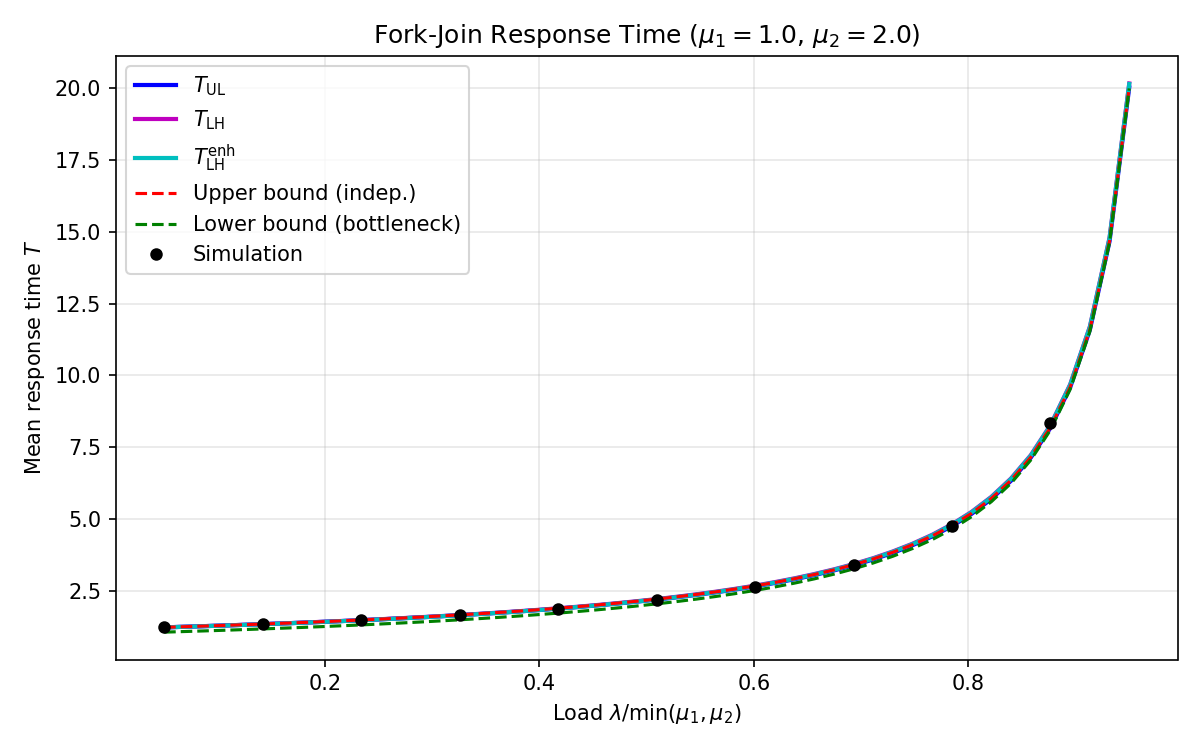
\includegraphics[width=0.85\textwidth]{figures/response_time_vs_load.png}
\caption{Mean response time vs.\ load $\lambda/\mumin$ for $\mu_1 = 1.0$,
         $\mu_2 = 2.0$.
         Markers: simulation. Lines: approximations and bounds.}
\label{fig:vs-load}
\end{figure}

\begin{figure}[ht]
\centering
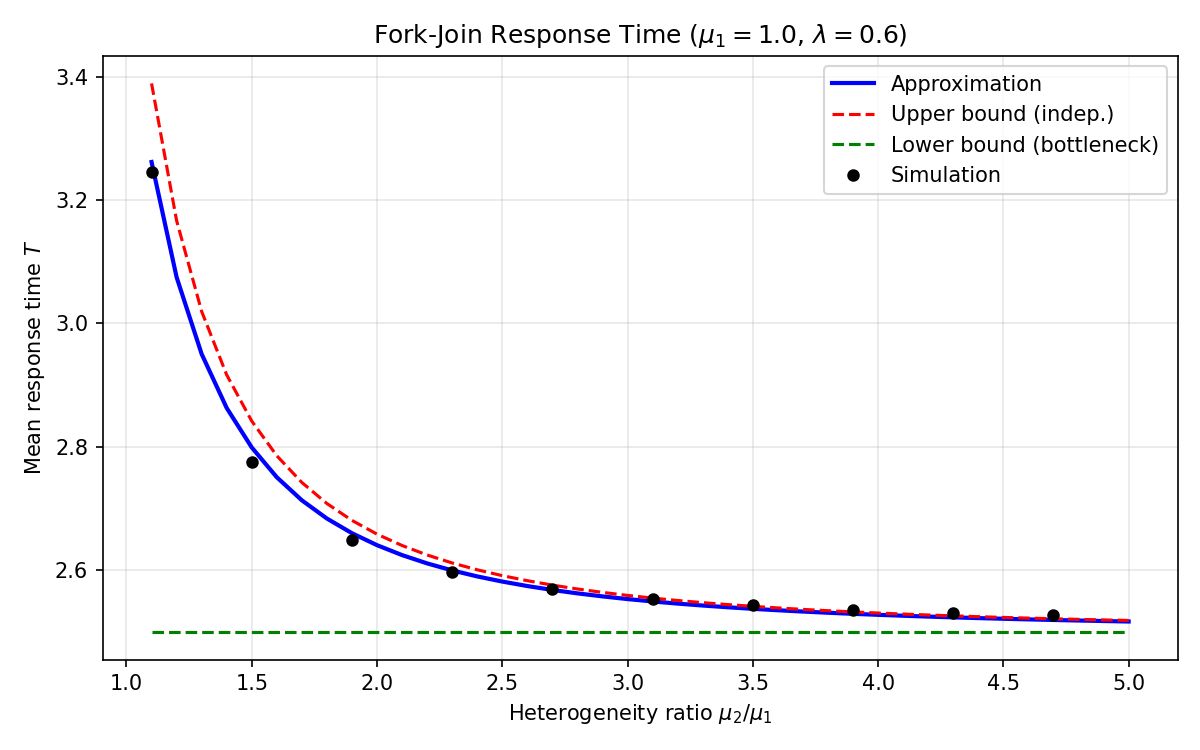
\includegraphics[width=0.85\textwidth]{figures/response_time_vs_heterogeneity.png}
\caption{Mean response time vs.\ heterogeneity ratio $\mu_2/\mu_1$ for
         $\mu_1 = 1.0$, $\lambda = 0.6$.
         Markers: simulation. Lines: approximations and bounds.}
\label{fig:vs-hetero}
\end{figure}

\subsection*{Sensitivity of $\Tul$ to Heterogeneity and Load}

Among the three approximations, $\Tul$ achieves the best uniform accuracy across
all loads and heterogeneity ratios, remains within the theoretical bounds by
construction, and requires no tunable parameters.
To characterize how its accuracy depends on both dimensions simultaneously,
we sweep the heterogeneity ratio $r = \mu_2/\mu_1$ from 1 to 8 across four
load levels chosen with a geometric spacing in the slack to saturation,
$1 - \rho \in \{0.48, 0.24, 0.12, 0.06\}$, i.e.\ $\rho \in \{0.52, 0.76, 0.88, 0.94\}$.

The heterogeneity grid uses 8 values $r \in \{1, 1.15, 1.3, 1.5, 2, 3, 5, 8\}$,
spaced more densely near $r = 1$ where $T$ transitions most steeply from
the homogeneous value to the bottleneck asymptote.
Each of the 32 simulation points uses 10\,M jobs with a 500\,K-job warmup
and a single random seed; 95\% confidence intervals are computed by the
normal approximation.

Figure~\ref{fig:tul-hetero-panel} shows the results.
At all four load levels, $\Tul$ closely tracks the simulation.
Most of the descent from the homogeneous value to the bottleneck plateau occurs
in $r \in [1, 2]$; beyond $r \approx 3$ the curves are essentially flat.
The relative error (right axis) peaks near $r = 1.15$--$1.3$ and is bounded
below $1.3\%$ for $\rho \leq 0.88$, consistent with the worst-case error of
$+1.13\%$ reported in Table~\ref{tab:results}.
At the highest load ($\rho = 0.94$), the single-seed estimate at $r = 1$
lies slightly above the exact homogeneous value, a reminder that estimates near
saturation require either multiple seeds or substantially longer runs to
eliminate transient bias; the displayed CI underestimates the true uncertainty
in this regime because consecutive response times are highly correlated near
saturation.

\begin{figure}[!ht]
\centering
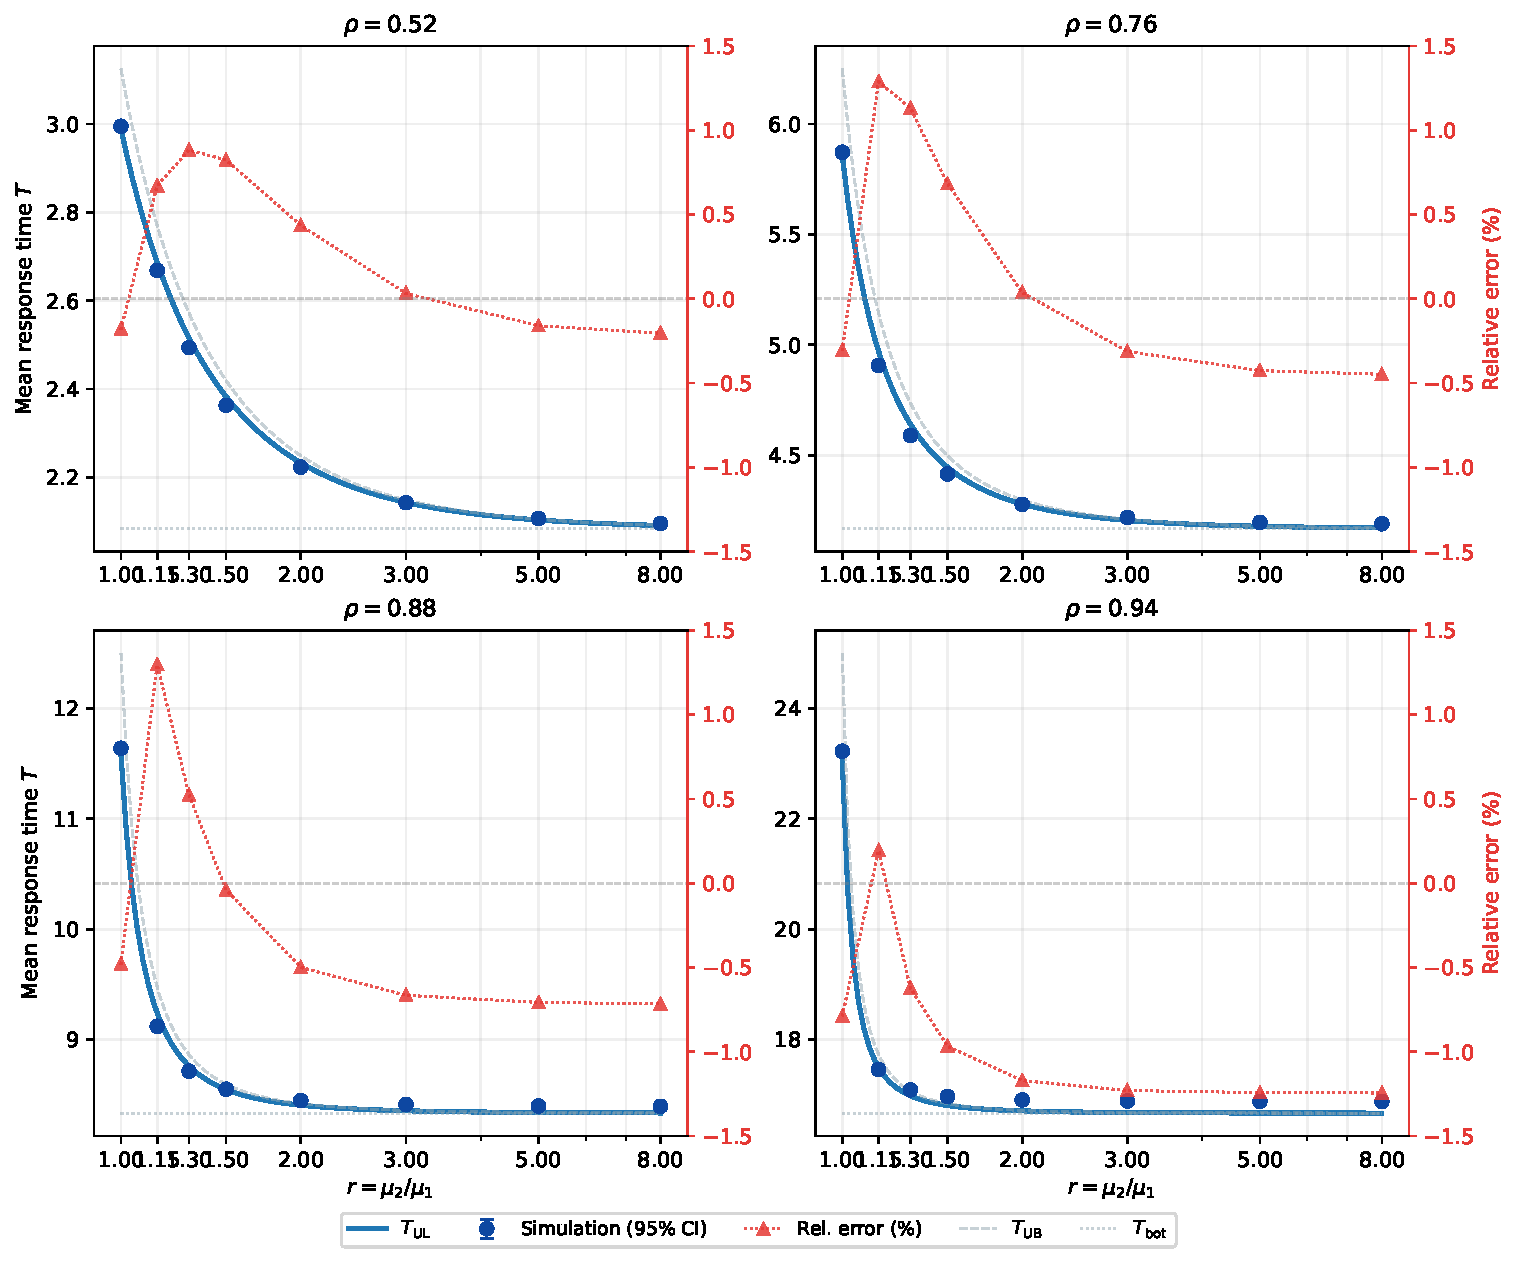
\includegraphics[width=\textwidth]{figures/t_ul_vs_heterogeneity.pdf}
\caption{$\Tul$ vs.\ heterogeneity ratio $r = \mumax/\mumin$ for four load
         levels $\rho \in \{0.52, 0.76, 0.88, 0.94\}$.
         Solid blue line: $\Tul$ (analytical); filled circles: simulation
         with 95\,\% CI bars ($10\,\mathrm{M}$ jobs, seed\,=\,42).
         Dashed and dotted gray lines: upper bound $\Tub$ and lower bound
         $\Tbot$.
         Right axis (red triangles): relative error
         $(\Tul - \Tsim)/\Tsim \times 100\%$.}
\label{fig:tul-hetero-panel}
\end{figure}

\subsection*{Enhanced LH Approximation}

Table~\ref{tab:results-lhe} compares $\Tlh$ and $\Tlhe$ against simulation.
Both use $\beta = 10$.

\begin{table}[ht]
\centering
\caption{$\Tlh$ vs.\ $\Tlhe$ vs.\ simulation for heterogeneous two-queue fork-join.
         $\Tsim$ and 95\% CI as in Table~\ref{tab:results}.
         Errors are $(T_{\text{approx}} - \Tsim)/\Tsim \times 100\%$.}
\label{tab:results-lhe}
\resizebox{\textwidth}{!}{%
\begin{tabular}{@{}cccccccccc@{}}
\toprule
$\mu_1$ & $\mu_2$ & $\lambda$ & $\rho_1$
        & $\Tsim$ & $\pm$95\%\,CI & $\Tlh$ & Err & $\Tlhe$ & Err \\
\midrule
1.0 & 1.0 & 0.3 & 0.30 & 2.089 & 0.001 & 2.089 & $0.00\%$ & 2.089 & $0.00\%$ \\
1.0 & 1.0 & 0.6 & 0.60 & 3.562 & 0.004 & 3.562 & $+0.01\%$ & 3.562 & $+0.01\%$ \\
1.0 & 1.0 & 0.9 & 0.90 & 13.892 & 0.082 & 13.875 & $-0.12\%$ & 13.875 & $-0.12\%$ \\
\midrule
1.0 & 1.5 & 0.3 & 0.30 & 1.707 & 0.001 & 1.698 & $-0.51\%$ & 1.710 & $+0.21\%$ \\
1.0 & 1.5 & 0.6 & 0.60 & 2.768 & 0.003 & 2.776 & $+0.31\%$ & 2.801 & $+1.20\%$ \\
1.0 & 1.5 & 0.9 & 0.90 & 10.142 & 0.083 & 10.325 & $+1.80\%$ & 10.362 & $+2.17\%$ \\
\midrule
1.0 & 2.0 & 0.3 & 0.30 & 1.583 & 0.001 & 1.595 & $+0.75\%$ & 1.589 & $+0.34\%$ \\
1.0 & 2.0 & 0.6 & 0.60 & 2.624 & 0.003 & 2.667 & $+1.64\%$ & 2.654 & $+1.14\%$ \\
1.0 & 2.0 & 0.9 & 0.90 & 10.050 & 0.083 & 10.170 & $+1.19\%$ & 10.150 & $+0.99\%$ \\
\midrule
1.0 & 3.0 & 0.6 & 0.60 & 2.548 & 0.003 & 2.583 & $+1.39\%$ & 2.561 & $+0.51\%$ \\
1.0 & 5.0 & 0.6 & 0.60 & 2.516 & 0.003 & 2.533 & $+0.68\%$ & 2.519 & $+0.13\%$ \\
\bottomrule
\end{tabular}%
}
\end{table}

\paragraph{Homogeneous case ($\mu_1 = \mu_2 = 1.0$).}
As proved in Section~\ref{sec:approx-lhe}, the quadratic coefficient $c_2 = 0$
when $r = 1$, so $\Tlhe \equiv \Tlh$.
Both recover Nelson--Tantawi exactly; residual errors ($\leq 0.12\%$) are
simulation noise.

\paragraph{Moderate heterogeneity ($r = 1.5$).}
$\Tlhe$ is slightly less accurate than $\Tlh$ across all loads
(worst case $+2.17\%$ vs.\ $+1.80\%$ at heavy load).
This regime is where the power-law model $h(r) = 1 + \tfrac{3}{8}r^{-\beta}$
is least reliable: $h(r)$ varies steeply near $r = 1$, and the resulting
systematic error in the heavy-traffic anchor dominates the benefit of
matching the first derivative.
Both LH variants are therefore less accurate than $\Tul$ ($+0.50\%$) in
this regime.

\paragraph{High heterogeneity ($r \geq 2$).}
$\Tlhe$ consistently outperforms $\Tlh$:
at $r = 2$ and $\lambda \in \{0.3, 0.6\}$ errors fall from $+0.75\%,\,+1.64\%$
to $+0.34\%,\,+1.14\%$; at $r = 3$ from $+1.39\%$ to $+0.51\%$;
and at $r = 5$ from $+0.68\%$ to $+0.13\%$.
In this regime $h(r) \approx 1$ and the first light-traffic derivative
$T_0'$ carries meaningful information about the service-time
heterogeneity that improves accuracy over a wide load range.

\section{Discussion}
\label{sec:discussion}

\subsection{Intuition}

The interpolation weight $\alpha = \bar{\rho}/4$ captures the effect of queueing correlation. At low load, tasks rarely queue, so their sojourn times are nearly independent and the upper bound is tight. As load increases, tasks experience correlated waiting due to the shared arrival stream, which reduces the synchronization overhead and pulls the response time toward the bottleneck.

The factor of $1/4$ in $\alpha$ is inherited from the homogeneous case analysis. In the homogeneous setting, the synchronization delay is $\text{Sync} = (4-\rho)/[8(\mu-\lambda)]$~\citep{Nelson1988}, and the independent synchronization delay would be $1/[2(\mu-\lambda)]$. Their ratio at $\rho = 1$ determines the interpolation scaling.

\subsection{Comparison with Other Approaches}

Table~\ref{tab:comparison} summarizes existing approaches for fork-join response time analysis.

\begin{table}[ht]
\centering
\caption{Comparison of approaches for fork-join mean response time.}
\label{tab:comparison}
\begin{tabular}{@{}llcc@{}}
\toprule
Approach & Type & Closed-form? & Heterogeneous? \\
\midrule
Nelson--Tantawi~\citep{Nelson1988} & Approximation & Yes & No \\
Flatto--Hahn~\citep{Flatto1984,Flatto1985} & Exact (gen.\ func.) & No & Yes \\
Ko--Serfozo~\citep{Ko2004} & Bounds & Semi & Yes \\
Kemper--Mandjes~\citep{Kemper2012} & Bounds + heavy traffic & Semi & Yes \\
Rizk et al.~\citep{Rizk2015} & Distributional bounds & Semi & Yes \\
Varki~\citep{Varki2001} & Split-merge (M/G/1) & Yes & Yes (UB for FJ) \\
\textbf{This work} & \textbf{Interpolation approx.} & \textbf{Yes} & \textbf{Yes} \\
\bottomrule
\end{tabular}
\end{table}

Our approximation fills a gap: it is the only directly evaluable closed-form expression for heterogeneous fork-join (not split-merge) that is exact in the homogeneous limit and respects known bounds.

\subsection{Limitations}

\begin{itemize}
\item The formula is a heuristic approximation, not an exact result. The weight $\alpha = \bar{\rho}/4$ is a natural generalization from the homogeneous case but is not derived from first principles for the heterogeneous setting.
\item The approximation consistently overestimates the true response time by up to ${\sim}2$\%, with the largest errors at moderate heterogeneity ($\mu_2/\mu_1 \approx 1.5$) under heavy load. This suggests the correlation correction could be slightly stronger in the heterogeneous case.
\item Further validation against numerical inversion of the Flatto--Hahn generating function could provide exact reference values for calibration.
\end{itemize}

\section{Conclusion}
\label{sec:conclusion}

We have presented two closed-form approximations for the mean response time
of a heterogeneous two-queue M/M/1 fork-join system with service rates
$\mu_1 \geq \mu_2$ and Poisson arrival rate $\lambda$.

The first, the \emph{upper-lower bound interpolation}:
\begin{equation}
  \Tul = \left(1 - \frac{\rho_1+\rho_2}{8}\right)\Tub
          + \frac{\rho_1+\rho_2}{8}\,\Tbot,
\end{equation}
is a parameter-free convex combination of the independent upper bound and
the bottleneck lower bound, always within the bounds, with errors below $1.2\%$.

The second, the \emph{light-heavy traffic interpolation}:
\begin{equation}
  \Tlh = \frac{\mumin T_0 + \bigl(h(r) - \mumin T_0\bigr)\rho}
              {\mumin - \lambda},
  \qquad h(r) = 1 + \frac{3}{8}\,r^{-\beta},
\end{equation}
is grounded in the Reiman--Simon framework, matching the exact light-traffic
value and a heterogeneity-adjusted heavy-traffic limit, with errors below $2.5\%$.

Both approximations recover the Nelson--Tantawi exact formula in the homogeneous
case, exhibit the correct singularity in heavy traffic, and are validated
against simulation to within $2.5\%$ across a wide range of loads and
heterogeneity levels.

Future directions include: (i)~extending $\Tlh$ to a quadratic Reiman--Simon
numerator by computing the first light-traffic derivative $f'(0)$,
which may further reduce errors and enable an analytic determination of $\beta$;
(ii)~deriving the slope $\partial h/\partial r|_{r=1}$ from a perturbation
analysis of the Flatto--Hahn generating function, which would close $\beta$
without requiring simulation calibration; and
(iii)~extending both methods to systems with more than two servers.


\bibliographystyle{abbrv}
\bibliography{references}

\end{document}
